% ****** Start of file apssamp.tex ******
%
%   This file is part of the APS files in the REVTeX 4.1 distribution.
%   Version 4.1r of REVTeX, August 2010
%
%   Copyright (c) 2009, 2010 The American Physical Society.
%
%   See the REVTeX 4 README file for restrictions and more information.
%
% TeX'ing this file requires that you have AMS-LaTeX 2.0 installed
% as well as the rest of the prerequisites for REVTeX 4.1
%
% See the REVTeX 4 README file
% It also requires running BibTeX. The commands are as follows:
%
%  1)  latex apssamp.tex
%  2)  bibtex apssamp
%  3)  latex apssamp.tex
%  4)  latex apssamp.tex
%
\documentclass[%
 reprint,
 superscriptaddress,
%groupedaddress,
%unsortedaddress,
%runinaddress,
%frontmatterverbose, 
%preprint,
%showpacs,preprintnumbers,
%nofootinbib,
%nobibnotes,
%bibnotes,
 amsmath,amssymb,
 %aps,
pra,
%prb,
%rmp,
%prstab,
%prstper,
%floatfix,
]{revtex4-1}

\usepackage{graphicx}% Include figure files
\usepackage{dcolumn}% Align table columns on decimal point
\usepackage{cancel}
\usepackage{tikz}
\usepackage{pgfplots}
\pgfplotsset{compat=1.13}
\setcitestyle{square}

\usepackage{bm}% bold math
\usepackage{verbatim}
%\usepackage{hyperref}% add hypertext capabilities
%\usepackage[mathlines]{lineno}% Enable numbering of text and display math
%\linenumbers\relax % Commence numbering lines

%\usepackage[showframe,%Uncomment any one of the following lines to test 
%%scale=0.7, marginratio={1:1, 2:3}, ignoreall,% default settings
%%text={7in,10in},centering,
%%margin=1.5in,
%%total={6.5in,8.75in}, top=1.2in, left=0.9in, includefoot,
%%height=10in,a5paper,hmargin={3cm,0.8in},
%]{geometry}

\begin{document}

%\preprint{APS/123-QED}

%\thanks{A footnote to the article title}%
\title{Dye sensitized solar cell (DSC)}

\author{Ahmad Fahad}
\email{ahmad.fahad@tum.de}
\affiliation{%
 Department of Electrical and Computer Engineering, Technical University of Munich, Arcisstra{\ss}e 21, 80333 Munich, Germany
}%

\date{\today}% It is always \today, today,
             %  but any date may be explicitly specified

\begin{abstract}
%Please use this \LaTeX{} template to structure your report. The structure below is commonly used for scientific paper writing. We recommend to try to keep to this structure in order to practice scientific writing. Please do not exceed 4 pages, additional information like parts of the code can be added in the appendix (does not count to the 4 pages).
\end{abstract}

\pacs{Valid PACS appear here}% PACS, the Physics and Astronomy
                             % Classification Scheme.
%\keywords{Suggested keywords}%Use showkeys class option if keyword
                              %display desired
\maketitle

%\tableofcontents


\section{Introduction}
\label{sec:introduction}

The future of new Solar Cells could be the DYE Solar Cell technique which works with a liquid electrolyte between the Anode and Cathode instead of Silicium like in a typical Solar Cell. Improving this technique will lead to a lot new inventions in energy harvesting and will be a big application to a lot of electronical devices.

This Simulation should show the influence of different parameters to the DYE cell and to get a basic knowledge of the TiberCAD program.

\section{Methods}
\label{sec:methods}

To get an overview and a basic knowledge of the DYE Solar Cell it is simulated with the TiberCAD program \ref{fig:DYE_Sim}. The values of the simulation are used to visualize the emission spectrum and the absorption function of the wavelength. Further on the I-V-curve is shown in order of a different voltage range. The short current condition of an Iodide, Triodide, the electrostatic potential and the illumination intensity are put into Graphs. Afterwards the simulation will be done again with different values of the kinetic rate, the prosity and illumination. The results will be shown in I-V-curves and the fill factor such as the power efficiency will be calculated.  
\\ 
\begin{figure}[h]
	\centering
	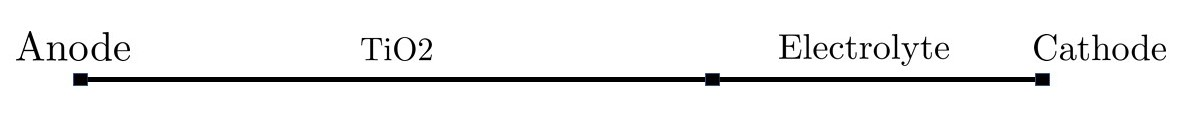
\includegraphics[width=\columnwidth]{grafik/DYE_Sim}
	\caption{Labeled DYE Cell in TiberCAD}
	\label{fig:DYE_Sim}
\end{figure}

\subsection*{Example Equation}
In Born-Oppenheimer approximation, the electron and nuclei motion is separated. The Hamiltonian of a many-particle system, e.g. a molecule, is given by
\begin{equation}
\label{eq:example_equation}
    \hat{H} = \sum_i \frac{\hbar^2}{2m}\nabla_i^2 - \sum_{i<j}\frac{e^2}{r_{ij}} + \sum_{i}\sum_{k}\frac{e^2 Z_{k}}{r_{ij}} \,,
\end{equation}
where $\hbar$ is the reduced Planck's constant, $m$ is the electron mass, \dots 

We can refer to the example equation using the reference command: See eq. (\ref{eq:example_equation}).

\section{Results}
\label{sec:results}

What's the answer? Put the result there, in numbers. Plot your results including all important facts, label the axis, show a legend, and give an explanation to the obtained results.

\subsection*{Example Figure}

In Fig. \ref{fig:C60_molecular_orbitals} the molecular orbitals for the C60 molecule are shown. 

\begin{figure}[h]
    \centering
    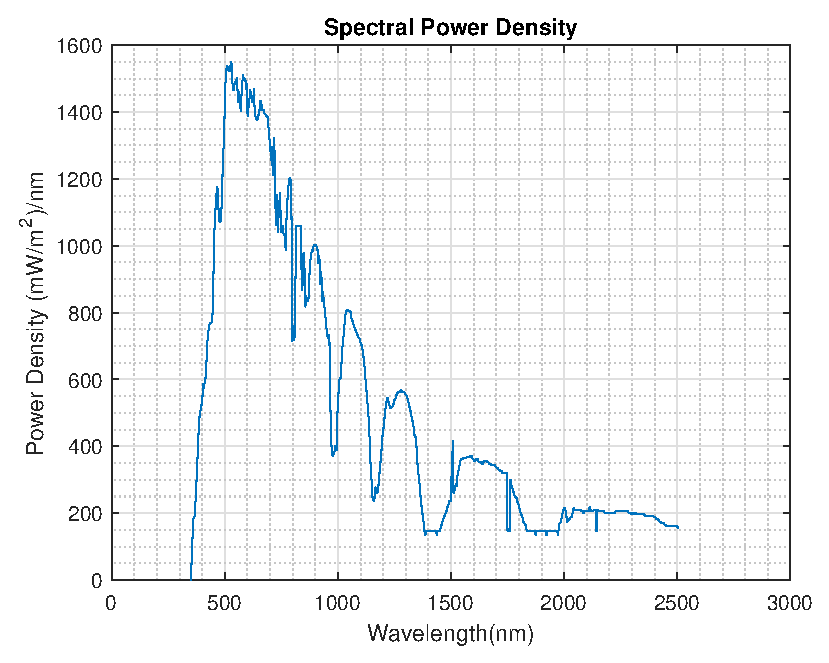
\includegraphics[width=\columnwidth]{Figures_eps/SpectralPowerDensity.eps}
    \caption{SpectralPowerDensity}
    \label{fig:C60_molecular_orbitals}
\end{figure}

\begin{figure}[h]
    \centering
    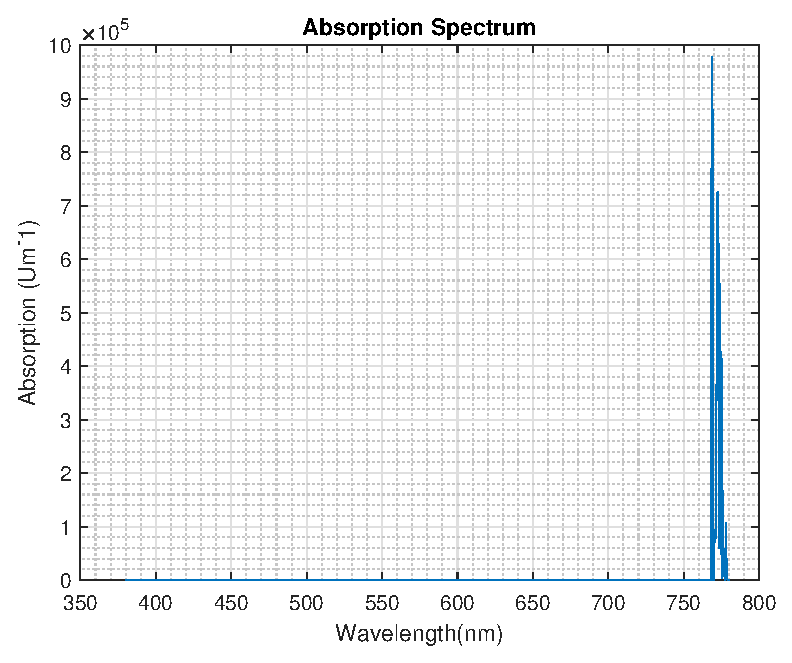
\includegraphics[width=\columnwidth]{Figures_eps/AbsorptionSpectrum.eps}
    \caption{AbsorptionSpectrum}
    \label{fig:C60_molecular_orbitals}
\end{figure}

\subsection*{Example Citation}

An introduction to quantum mechanics is given by \cite{griffiths2016introduction}.

\section{Conclusion}
\label{sec:conclusion}
What are the implications of your answer? Are your results general, potentially generalizable, or specific to a particular case?

\section*{Appendix}
Additional information and codes.

\bibliographystyle{apsrev4-1}
\bibliography{references}

% \pagebreak

\end{document}
%
% ****** End of file apssamp.tex ******
